\documentclass[11pt]{article}

\usepackage[T1]{fontenc}
\usepackage[utf8]{inputenc}
\usepackage{lmodern}
\usepackage[margin=1in]{geometry}
\usepackage{microtype}
\usepackage{amsmath,amssymb,amsthm,mathtools}
\usepackage{booktabs,array,longtable}
\usepackage{enumitem}
\usepackage{xcolor}
\usepackage{tikz}
\usetikzlibrary{arrows.meta,calc,positioning}
\usepackage{listings}
\usepackage{hyperref}
\usepackage[nameinlink,noabbrev]{cleveref}

\definecolor{deepblue}{RGB}{28,62,105}
\definecolor{softblue}{RGB}{235,242,250}
\definecolor{softgray}{RGB}{246,247,249}
\definecolor{darkgreen}{RGB}{25,105,70}
\hypersetup{
  colorlinks=true,
  linkcolor=deepblue,
  citecolor=deepblue,
  urlcolor=deepblue,
  pdftitle={Farthest Surface Points and the Intrinsic Diameter of a Cuboid},
  pdfauthor={Prepared for Vladimir Reshetnikov}
}

\newtheorem{theorem}{Theorem}[section]
\newtheorem{lemma}[theorem]{Lemma}
\newtheorem{proposition}[theorem]{Proposition}
\newtheorem{corollary}[theorem]{Corollary}
\theoremstyle{definition}
\newtheorem{definition}[theorem]{Definition}
\newtheorem{remark}[theorem]{Remark}

\newcommand{\R}{\mathbb{R}}
\newcommand{\Surf}{\partial\mathcal B}
\newcommand{\distS}{d_{\Surf}}
\newcommand{\diamS}{\operatorname{diam}_{\Surf}}
\newcommand{\sq}{^{2}}
\newcommand{\dd}{\,\mathrm d}
\DeclareMathOperator{\argmax}{arg\,max}

\lstset{
  basicstyle=\ttfamily\small,
  backgroundcolor=\color{softgray},
  frame=single,
  rulecolor=\color{gray!35},
  breaklines=true,
  columns=fullflexible,
  keepspaces=true
}

\title{\textbf{Farthest Surface Points and the Intrinsic Diameter of a Cuboid}\\
\large Exact coordinates, exact lengths, proof, and a Lean formalization plan}
\author{Prepared for Vladimir Reshetnikov}
\date{19 November 2026}

\begin{document}
\maketitle

\begin{abstract}
Let a cuboid have positive side lengths $a,b,c$, and let distance mean the
length of the shortest path constrained to the cuboid surface.  This report
solves two different maximin problems.  First, with a vertex $X$ fixed, it
gives an explicit farthest point $Y$ and the exact intrinsic distance
$\distS(X,Y)$.  The answer has two regimes: the opposite vertex is optimal for
moderately shaped boxes, but for sufficiently elongated boxes the maximizer
moves into the face opposite the longest edge.  Second, when both endpoints
are free, it gives the complete three-regime formula for the intrinsic
diameter, including coordinates of a diametral pair.  In the third regime the
answer is the unique root of a strictly increasing one-variable radical
equation.  The freely chosen endpoints give a strictly longer shortest path
exactly outside an explicit region $\mathcal M_E$; inside that region there is
no improvement over a fixed vertex.  The proof reduces the surface metric to
finite planar unfoldings and then performs exact semialgebraic optimization.
A Lean blueprint, concrete algebra file, executable calculator, and symbolic
and numerical validation scripts accompany the paper.
\end{abstract}

\tableofcontents

\section{Statement of the answers}

\subsection{Normalization}

The formulas are clearest after sorting the three side lengths.  Let
\begin{equation}\label{eq:sort}
  0<A\le B\le C
\end{equation}
be the numbers $a,b,c$ in nondecreasing order, and use coordinates on
\begin{equation}
  \mathcal B=[0,A]\times[0,B]\times[0,C].
\end{equation}
The coordinate along the longest edge is therefore the third coordinate.
Section~\ref{sec:transport} explains how to undo the axis permutation and how
to handle an arbitrary selected vertex.

Put
\begin{equation}\label{eq:L0}
  L_0:=\sqrt{(A+B)^2+C^2}.
\end{equation}
This is the intrinsic distance between opposite vertices: unfold two adjacent
side lengths into a segment of length $A+B$, leaving the third side $C$
orthogonal to it.

\subsection{A fixed selected vertex}

Take $X=(0,0,0)$ and define
\begin{equation}\label{eq:KdeltaR}
\begin{split}
  K&:=2C^2-2BC-AC-AB,\\
  \delta&:=\frac{A(C-B)}{2C},\\
  R^2&:=\frac{(B^2+C^2)(A^2+2AC+2C^2)}{2C^2}.
\end{split}
\end{equation}

\begin{theorem}[Farthest point from a vertex]\label{thm:fixed-summary}
For the surface metric of $\mathcal B$:
\begin{enumerate}[label=\textup{(\roman*)}]
\item If $K\le 0$, one may take
\[
  Y=(A,B,C),\qquad \distS(X,Y)=L_0.
\]
\item If $K>0$, one may take
\[
  Y=(A-\delta,B-\delta,C),\qquad \distS(X,Y)=R.
\]
\end{enumerate}
Equivalently, the eccentricity of a vertex is $\max\{L_0,R\}$, because
\begin{equation}\label{eq:fixed-gap}
  R^2-L_0^2=\frac{A(C-B)}{2C^2}\,K.
\end{equation}
At $K=0$, both displayed points attain the same maximum.
\end{theorem}

Thus, for a $1\times1\times2$ box, the farthest point from $(0,0,0)$ is
$(3/4,3/4,2)$, not $(1,1,2)$.

\subsection{Both endpoints free}

Define
\begin{equation}\label{eq:alpha-beta}
\begin{split}
 \alpha&:=\sqrt{\max\{0,A^2+2AB-2BC\}},\\
 \beta&:=\sqrt{\max\{0,B^2+2AB-2AC\}}.
\end{split}
\end{equation}
The ``opposite-vertex region'' is
\begin{equation}\label{eq:ME}
  \mathcal M_E:\qquad \alpha+\beta\ge 2C-A-B.
\end{equation}
Also put
\begin{equation}\label{eq:Q}
  Q:=A^2B^2-C^2(B-A)(A+B+2C).
\end{equation}

\begin{theorem}[Intrinsic diameter and a diametral pair]\label{thm:diam-summary}
Let $D=\diamS(\Surf)$.  Exactly one of the following mutually exclusive rules
(with the indicated convention at $Q=0$) gives a diametral pair.

\medskip
\noindent\textbf{I. Opposite-vertex regime: $\mathcal M_E$.}
\[
  P=(0,0,0),\qquad Q_0=(A,B,C),\qquad D=L_0.
\]

\medskip
\noindent\textbf{II. Boundary-balancing regime: not $\mathcal M_E$ and $Q\le0$.}
Let
\begin{equation}\label{eq:Htau}
  H:=\sqrt{(B+C)^2-2A(C-B)-A^2},
  \qquad \tau:=\frac{B+C-H}{2}.
\end{equation}
Then
\begin{equation}\label{eq:boundary-pair}
  P=\left(\frac A2,\tau,0\right),\qquad
  Q_0=\left(\frac A2,B-\tau,C\right),
\end{equation}
and
\begin{equation}\label{eq:boundary-D}
  D^2=B^2+3C^2+2B(A+C)-2CH.
\end{equation}

\medskip
\noindent\textbf{III. Interior triple-balancing regime: not $\mathcal M_E$ and $Q>0$.}
There is a unique
\begin{equation}\label{eq:ell-domain}
  \ell\ge\max\{B+C,L_0\}
\end{equation}
solving
\begin{equation}\label{eq:root}
\boxed{
 \sqrt{\ell^2-(A+C)^2}
 +\sqrt{\ell^2-(B+C)^2}
 +\sqrt{2\ell^2-(A+B+C)^2}=C.}
\end{equation}
Set
\begin{equation}\label{eq:uvxy}
\begin{aligned}
  u&:=\sqrt{\ell^2-(B+C)^2}, &\qquad x_*&:=\frac{A-u}{2},\\
  v&:=\sqrt{\ell^2-(A+C)^2}, &\qquad y_*&:=\frac{B-v}{2}.
\end{aligned}
\end{equation}
Then
\begin{equation}\label{eq:interior-pair}
  P=(x_*,y_*,0),\qquad Q_0=(A-x_*,B-y_*,C),\qquad D=\ell.
\end{equation}
At $Q=0$, Cases II and III meet and give the same point and length.
\end{theorem}

The diameter formula in 
\cref{thm:diam-summary} was obtained by Nikonorov and Nikonorova
\cite{nikonorov2008diameter}.  The proof below is reorganized to expose the
finite unfolding formulas, the optimizing coordinates, and the direct
comparison with the fixed-vertex problem.

\begin{corollary}[Does freeing both endpoints help?]\label{cor:comparison}
Let $E$ be the largest surface distance from a selected vertex, as in
\cref{thm:fixed-summary}.  Then
\[
  D=E=L_0 \quad\Longleftrightarrow\quad (A,B,C)\in\mathcal M_E.
\]
Outside $\mathcal M_E$ one has the strict inequality $D>E$.
\end{corollary}

So the answer is: \emph{sometimes}.  Freeing both endpoints gives no gain in
$\mathcal M_E$, and gives a strict gain everywhere else.

\section{The intrinsic metric and planar unfoldings}

A surface path is a continuous map $\gamma:[0,1]\to\Surf$.  Its length is the
usual supremum over polygonal variations,
\begin{equation}\label{eq:pathlength}
  L(\gamma)=\sup_{0=t_0<\cdots<t_n=1}
  \sum_{i=1}^n \lVert\gamma(t_i)-\gamma(t_{i-1})\rVert_2,
\end{equation}
and
\begin{equation}\label{eq:intrinsic}
  \distS(P,Q)=\inf\{L(\gamma):\gamma(0)=P,\ \gamma(1)=Q,
  \ \gamma([0,1])\subseteq\Surf\}.
\end{equation}
This definition excludes any chord through the cuboid interior.

A shortest path on a polyhedral surface is a polygonal line.  Whenever its
successive faces are unfolded into one plane, the path becomes a straight
segment.  Conversely, a straight segment in a valid unfolding folds back to a
surface path of the same length.  A shortest path never needs to revisit the
interior of a face: after unfolding, the portion between the first and last
visits could be replaced by a straight segment.  Hence only finitely many
reduced face chains need be considered.  This is the geometric reason that
both problems reduce to minima of finitely many Euclidean distances; compare
the general polyhedral algorithms in \cite{orourke1989geodesic}.

\section{The fixed-vertex problem}\label{sec:fixed-proof}

Throughout this section, $X=(0,0,0)$.

\subsection{Only the top face can beat the opposite vertex}

\begin{lemma}\label{lem:not-top}
If $Z\in\Surf$ does not lie in the top face $z=C$, then
$\distS(X,Z)\le L_0$.
\end{lemma}

\begin{proof}
On the three faces incident with $X$, the direct face segment gives respectively
lengths at most $\sqrt{A^2+B^2}$, $\sqrt{A^2+C^2}$, and
$\sqrt{B^2+C^2}$, all below $L_0$.  On the face $x=A$, unfold that face with
the bottom face.  A point $(A,y,z)$ is then reached by a planar segment of
length
\[
  \sqrt{(A+y)^2+z^2}\le\sqrt{(A+B)^2+C^2}=L_0.
\]
The face $y=B$ is identical after exchanging $A$ and $B$.  These five faces
are precisely the complement of the relative interior of $z=C$.
\end{proof}

\subsection{Four source images on the top face}

Write a top-face point as $Z=(p,q,C)$ with
$0\le p\le A$, $0\le q\le B$.  Unfolding the reduced face chains from $X$ to
the top face gives four relevant images of $X$ in the top-face plane:
\begin{equation}\label{eq:sources}
  S_1=(-C,0),\quad S_2=(A+C,-A),\quad
  S_3=(0,-C),\quad S_4=(-B,B+C).
\end{equation}
The first and third correspond to crossing one vertical face.  The second and
fourth correspond to passing across the bottom and the opposite vertical
face.  Here is a finite completeness check, included to avoid hiding anything
in the phrase ``all unfoldings.''  By the face-straightening observation of the
previous section, a shortest path may be chosen with a simple face sequence.
Enumerate the simple paths in the six-vertex face-adjacency graph, starting in
one of the three faces $x=0$, $y=0$, $z=0$ incident with $X$ and ending at
$z=C$.  There are $80$ such sequences and, after unfolding, only $28$
distinct planar images of $X$.  Four are the sites in \eqref{eq:sources}.

Every one of the other $24$ images $T$ is dominated throughout the top-face
rectangle by one of the four canonical sites: for a suitable $i$,
\[
  \lVert(p,q)-S_i\rVert^2\le \lVert(p,q)-T\rVert^2
  \qquad(0\le p\le A,\ 0\le q\le B).
\]
Indeed, the difference of the right and left sides is affine in $(p,q)$, so it
suffices to check the four rectangle corners.  Writing
$B=A+u$ and $C=A+u+v$ with $u,v\ge0$, all $24\times4$ corner differences
expand as polynomials in $A,u,v$ with nonnegative coefficients.  The exact
source list, the chosen dominator, and every corner polynomial are generated
by \texttt{scripts/audit\_unfoldings.py} and recorded in
\texttt{UNFOLDING\_AUDIT.txt}.

There is one remaining validity point: a planar segment must cross the edges
of its chosen net in the intended order.  The nets for $S_1$ and $S_3$ are
valid for every $(p,q)$ in the top rectangle.  The net for $S_2$ is valid
exactly when
\[
  Ap+Cq\ge A^2.
\]
Whenever $S_2$ can be nearest, comparison with $S_3$ gives
\[
  (A+C)p+(C-A)q\ge A(A+C),
\]
and hence
\[
 Ap+Cq-A^2\ge \frac{A^2+C^2}{A+C}\,q\ge0.
\]
Similarly, the $S_4$ net is valid exactly when $Cp+Bq\ge B^2$; whenever $S_4$
is no farther than $S_1$, one has
\[
 q\ge B-\frac{C-B}{B+C}p,
 \qquad
 Cp+Bq-B^2\ge\frac{B^2+C^2}{B+C}\,p\ge0.
\]
Thus whichever canonical image realizes the minimum supplies an actual
surface path, while all noncanonical images are globally dominated.
Consequently,
\begin{equation}\label{eq:top-min}
  \distS(X,Z)^2=\min_{1\le i\le4}\lVert(p,q)-S_i\rVert_2^2.
\end{equation}

\begin{figure}[ht]
\centering
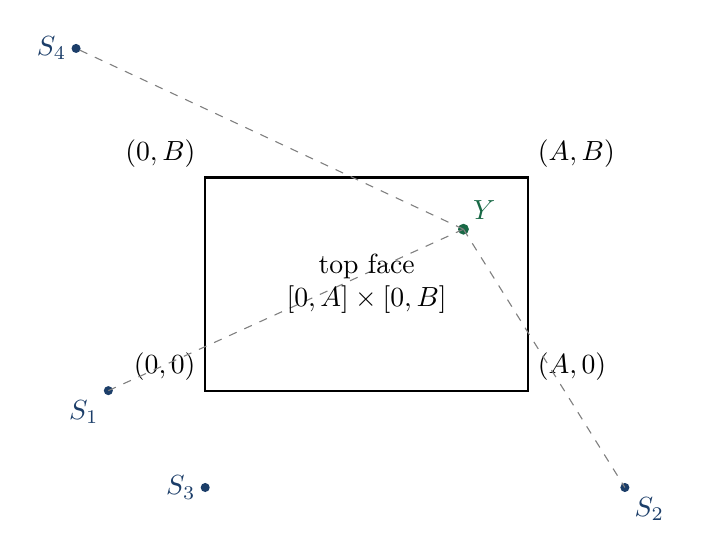
\begin{tikzpicture}[scale=0.82,>=Latex]
  \draw[thick] (0,0) rectangle (5,3.3);
  \node[above left] at (0,0) {$(0,0)$};
  \node[above right] at (5,0) {$(A,0)$};
  \node[above right] at (5,3.3) {$(A,B)$};
  \node[above left] at (0,3.3) {$(0,B)$};
  \fill[deepblue] (-1.5,0) circle (2pt) node[below left] {$S_1$};
  \fill[deepblue] (6.5,-1.5) circle (2pt) node[below right] {$S_2$};
  \fill[deepblue] (0,-1.5) circle (2pt) node[left] {$S_3$};
  \fill[deepblue] (-2,5.3) circle (2pt) node[left] {$S_4$};
  \fill[darkgreen] (4.0,2.5) circle (2.4pt) node[above right] {$Y$};
  \draw[dashed,gray] (4.0,2.5)--(-1.5,0);
  \draw[dashed,gray] (4.0,2.5)--(6.5,-1.5);
  \draw[dashed,gray] (4.0,2.5)--(-2,5.3);
  \node[align=center] at (2.5,1.65) {top face\\$[0,A]\times[0,B]$};
\end{tikzpicture}
\caption{The fixed-vertex problem becomes a farthest-nearest-site problem for
four source images in the plane of the top face.  The drawing is schematic,
not to scale.}
\label{fig:sources}
\end{figure}

\subsection{A finite Voronoi maximization}

Let
\[
  F(p,q):=\min_i\lVert(p,q)-S_i\rVert^2.
\]
Intersect the ordinary Voronoi cells of the four sites with the rectangle
$[0,A]\times[0,B]$.  Each cell is a convex polygon, because every inequality
$\lVert z-S_i\rVert^2\le\lVert z-S_j\rVert^2$ is affine in $z$.  On the
$i$th cell, $F(z)=\lVert z-S_i\rVert^2$, a convex quadratic.

\begin{lemma}[Convex maximum on a polygon]\label{lem:convex-poly}
A convex function on a compact polygon attains its maximum at a vertex of the
polygon.
\end{lemma}

\begin{proof}
Every point of the polygon is a convex combination of its vertices.  Convexity
bounds the function value by the same convex combination of the vertex
values, hence by their maximum.
\end{proof}

All Voronoi vertices on the rectangle boundary have $F\le L_0^2$.  Indeed:
\begin{align*}
 q=0 &: &&F(p,0)\le\lVert(p,0)-S_3\rVert^2=p^2+C^2\le L_0^2,\\
 p=0 &: &&F(0,q)\le\lVert(0,q)-S_1\rVert^2=q^2+C^2\le L_0^2,\\
 p=A &: &&F(A,q)\le\lVert(A,q)-S_2\rVert^2=C^2+(A+q)^2\le L_0^2,\\
 q=B &: &&F(p,B)\le\lVert(p,B)-S_4\rVert^2=C^2+(B+p)^2\le L_0^2.
\end{align*}
The corner $(A,B)$ attains $L_0^2$.

It remains to inspect interior intersections of three perpendicular
bisectors.  There are four formal triple circumcenters, but only two can be
vertices of the nearest-site Voronoi diagram.  The useful ones are
\begin{equation}\label{eq:T123}
  T_{123}=\left(\frac{A(A+C)}{2C},\frac{A(A+C)}{2C}\right)
\end{equation}
and
\begin{equation}\label{eq:T124}
  T_{124}=\left(\frac{A(B+C)}{2C},
  \frac{AB-AC+2BC}{2C}\right)=(A-\delta,B-\delta).
\end{equation}
Both points lie in the rectangle: for $T_{123}$ the common coordinate is
between $A/2$ and $A$ (and hence at most $B$), while for $T_{124}$ one has
$A/2\le A-\delta\le A$ and $0\le B-\delta\le B$.
Their common squared distances to the defining sites are
\begin{align}
 R_A^2&=\frac{(A^2+C^2)(A^2+2AC+2C^2)}{2C^2},\label{eq:RA}\\
 R^2&=\frac{(B^2+C^2)(A^2+2AC+2C^2)}{2C^2}.
\end{align}
At $T_{123}$, the omitted site $S_4$ is farther by
$2(B-A)(A+B+C)\ge0$.  At $T_{124}$, the omitted site $S_3$ is farther by
$2C(B-A)\ge0$.  Thus both are genuine nearest-site vertices.  For the other
two formal triple intersections, the omitted-site differences are
$2(A-B)(A+B+C)\le0$ and $2C(A-B)\le0$, so an omitted site is already closer;
except in degenerate ties, they are not Voronoi vertices.  Finally,
\begin{equation}\label{eq:RgeRA}
  R^2-R_A^2=
  \frac{(B-A)(A+B)(A^2+2AC+2C^2)}{2C^2}\ge0.
\end{equation}
By \cref{lem:convex-poly}, the top-face maximum is therefore
$\max\{L_0^2,R^2\}$.  Expanding gives the decisive factorization
\eqref{eq:fixed-gap}, completing the proof of \cref{thm:fixed-summary}.

\section{The intrinsic diameter}\label{sec:diam-proof}

\subsection{Central symmetry reduces two free points to two variables}

The cuboid surface is centrally symmetric under
\begin{equation}\label{eq:involution}
  I(x,y,z)=(A-x,B-y,C-z).
\end{equation}
We use one general theorem about centrally symmetric convex surfaces.

\begin{lemma}[Antipodal diameter theorem]\label{lem:antipodal}
If two points on a centrally symmetric convex surface realize its intrinsic
diameter, central symmetry exchanges the two points.
\end{lemma}

This is V\^{\i}lcu's theorem \cite{vilcu2000steinhaus}, used in precisely this
form in \cite{nikonorov2008diameter}.  It is the only global topological input
in the diameter proof.  Geometrically, a diametral pair consists of mutual
farthest points; on a centrally symmetric convex two-sphere, the cut-locus
separation forced at both endpoints is compatible with the fixed-point-free
central involution only when the endpoints are antipodes.

At least one endpoint of a diametral antipodal pair may be placed on a base
face.  Antipodal pairs lying only on profile faces have distance strictly less
than $L_0$, while opposite vertices already have distance $L_0$.  Reflections
in the two midplanes of the base then let us write every relevant pair as
\begin{equation}\label{eq:normalized-pair}
  M=(x,y,0),\qquad N=(A-x,B-y,C),
\end{equation}
with
\begin{equation}\label{eq:Omega}
  (x,y)\in\Omega:=[0,A/2]\times[0,B/2].
\end{equation}

\subsection{The five unfolding lengths}

A complete enumeration of reduced face chains for \eqref{eq:normalized-pair}
gives five candidate lengths:
\begin{align}
 d_1^2(x,y)&=(A+C)^2+(B-2y)^2,\label{eq:d1}\\
 d_2^2(x,y)&=(B+C)^2+(A-2x)^2,\label{eq:d2}\\
 d_3^2(x,y)&=(C+x+y)^2+(A+B-x-y)^2,\label{eq:d3}\\
 d_4^2(x,y)&=(A+B)^2+(C+2y)^2,\label{eq:d4}\\
 d_5^2(x,y)&=(A+B)^2+(C+2x)^2.\label{eq:d5}
\end{align}

For completeness, the face-chain classification is again finite and can be
checked without relying on a drawing.  A shortest path meets every face in a
connected set, hence has a simple face sequence.  There are $28$ simple paths
in the face-adjacency graph from the bottom face to the top face.  Unfolding
all of them gives $14$ distinct squared net lengths.  Five are
\eqref{eq:d1}--\eqref{eq:d5}.  To dispose of the other nine, put
\[
  \xi:=A-2x,\qquad \eta:=B-2y;
  \qquad 0\le\xi\le A,\quad 0\le\eta\le B.
\]
If $E_1,\ldots,E_9$ denote the nine noncanonical squared net lengths, exact
expansion gives the following dominance certificates:
\begin{center}
\begin{tabular}{ccl}
\toprule
net & dominated by & nonnegative difference\\
\midrule
$E_1$ & $d_3^2$ & $2\bigl((A+B)^2+(A+B+C)(\xi+\eta)\bigr)$\\
$E_2$ & $d_5^2$ & $4\xi(A+C)$\\
$E_3$ & $d_3^2$ & $2\bigl((A+B)(A+B-\eta)+\xi(A+B+C-\eta)\bigr)$\\
$E_4$ & $d_3^2$ & $2C(\xi+\eta)$\\
$E_5$ & $d_3^2$ & $2(A+B)(A+B-\xi-\eta)$\\
$E_6$ & $d_4^2$ & $4\eta(B+C)$\\
$E_7$ & $d_3^2$ & $2\xi(C-\eta)$\\
$E_8$ & $d_3^2$ & $2\bigl((A+B)(A+B-\xi)+\eta(A+B+C-\xi)\bigr)$\\
$E_9$ & $d_3^2$ & $2\eta(C-\xi)$\\
\bottomrule
\end{tabular}
\end{center}
Each expression is nonnegative under $0<A\le B\le C$ and the displayed
bounds on $\xi,\eta$.  The audit file lists the face sequence and full
polynomial for every $E_i$.  Therefore no omitted or formally invalid net can
lower the minimum.  Thus
\begin{equation}\label{eq:five-min}
  \distS(M,N)=\min_{1\le i\le5}d_i(x,y),
\end{equation}
and
\begin{equation}\label{eq:diam-maxmin}
  D=\max_{(x,y)\in\Omega}\min_i d_i(x,y).
\end{equation}
This is the exact maximin problem to solve.

\subsection{Exactly when opposite vertices are optimal}

At $(x,y)=(0,0)$, the minimum in \eqref{eq:five-min} equals $L_0$.
For $x,y>0$, $d_4,d_5>L_0$.  The other three inequalities factor as follows:
\begin{align}
 d_1^2-L_0^2&=2\bigl(y^2-By+\tfrac12A(C-B)\bigr),\label{eq:d1gap}\\
 d_2^2-L_0^2&=2\bigl(x^2-Ax+\tfrac12B(C-A)\bigr),\label{eq:d2gap}\\
 d_3^2-L_0^2&=2(x+y)(C-A-B+x+y).\label{eq:d3gap}
\end{align}
On the half-rectangle \eqref{eq:Omega}, the supremal admissible values
for the first two strict inequalities are
\[
  \sup\{y:d_1(x,y)>L_0\}=\frac{B-\beta}{2},\qquad
  \sup\{x:d_2(x,y)>L_0\}=\frac{A-\alpha}{2}.
\]
More explicitly, every smaller $y$ (respectively $x$) works.  If the
untruncated radicand defining $\beta$ (respectively $\alpha$) is negative,
the endpoint $B/2$ (respectively $A/2$) works as well; this harmless endpoint
distinction is why the supremum formulation is convenient.  Finally,
\[
 d_3>L_0\iff x+y>A+B-C,
\]
with the inequality automatic for positive $x+y$ when $A+B-C<0$.
The first two suprema can be approached simultaneously, and their sum is
$(A+B-\alpha-\beta)/2$.  Hence a point at which all five unfoldings exceed
$L_0$ exists exactly when
\[
  \frac{A+B-\alpha-\beta}{2}>A+B-C,
\]
that is,
\begin{equation}\label{eq:notME}
  \alpha+\beta<2C-A-B.
\end{equation}
This proves, without yet locating the maximizer, that
\begin{equation}\label{eq:Dbaseline}
  D=L_0\ \text{in }\mathcal M_E,
  \qquad D>L_0\ \text{outside }\mathcal M_E.
\end{equation}

\subsection{\texorpdfstring{The triple-balancing regime $Q>0$}{The triple-balancing regime Q > 0}}

Define two auxiliary functions by exact identities:
\begin{align}
 q_1(x,y)&:=\frac{2d_3^2-d_1^2-d_2^2}{8}\notag\\
 &=\left(x+\frac{C-A}{2}\right)
   \left(y+\frac{C-B}{2}\right)-\frac{C^2-AB}{4},\label{eq:q1}\\
 q_2(x,y)&:=\frac{d_1^2-d_2^2}{4}\notag\\
 &=\left(y-\frac B2\right)^2-
   \left(x-\frac A2\right)^2-
   \frac{(B-A)(A+B+2C)}4.\label{eq:q2}
\end{align}
The condition $d_1=d_2=d_3$ is exactly $q_1=q_2=0$.
Within $\Omega$, $q_1=0$ is the graph of the decreasing function
\begin{equation}\label{eq:L1graph}
 y=\frac{C^2-AB}{2(2x+C-A)}-\frac{C-B}{2},
\end{equation}
whereas $q_2=0$ is the graph of an increasing function (using the negative
square-root branch because $y\le B/2$).  Comparing their endpoint values gives
\begin{equation}\label{eq:intersectionQ}
 \text{a unique intersection }(x_*,y_*)\in\Omega
 \quad\Longleftrightarrow\quad Q\ge0.
\end{equation}
At $Q=0$ the intersection lies on $x=A/2$; for $Q>0$ it is an interior
triple-balancing point.

Let
\begin{equation}
  \ell=d_1(x_*,y_*)=d_2(x_*,y_*)=d_3(x_*,y_*).
\end{equation}
The remaining unfoldings do not undercut it.  The needed identities are
\begin{align}
 d_2^2-d_5^2
 &=-4(A+C)\left(x-\frac{B(C-A)}{2(A+C)}\right),\label{eq:d25}\\
 d_1^2-d_4^2
 &=-4(B+C)\left(y-\frac{A(C-B)}{2(B+C)}\right).\label{eq:d14}
\end{align}
The hyperbola intersection and $Q\ge0$ imply
\begin{equation}\label{eq:xy-lower}
  x_*\ge\frac{B(C-A)}{2(A+C)},\qquad
  y_*\ge\frac{A(C-B)}{2(B+C)}.
\end{equation}
For example, the second inequality follows from
$y_*\ge B(C-A)/(2C)$ on the decreasing graph \eqref{eq:L1graph}, followed by
\[
  \frac{B(C-A)}{2C}\ge\frac{A(C-B)}{2(B+C)},
\]
whose cleared numerator is $(B-A)C^2+B^2(C-A)\ge0$.  The first follows by
substituting the former bound into \eqref{eq:q2}; after squaring, the remaining
term is precisely controlled by $Q\ge0$.  Equations \eqref{eq:d25}--\eqref{eq:d14}
therefore yield $d_5\ge\ell$ and $d_4\ge\ell$, so the maximin value at the
intersection is indeed $\ell$.

To prove global optimality, set
\begin{equation}\label{eq:h}
  h(t):=(C+t)^2+(A+B-t)^2.
\end{equation}
Then $d_3^2(x,y)=h(x+y)$, and $h$ is strictly convex.  For any other point of
$\Omega$:
\begin{itemize}[leftmargin=2em]
\item if $x>x_*$, then $d_2(x,y)<\ell$ because $d_2$ decreases with $x$;
\item if $y>y_*$, then $d_1(x,y)<\ell$ because $d_1$ decreases with $y$;
\item otherwise, except at $(0,0)$ and $(x_*,y_*)$, one has
$0<x+y<x_*+y_*$.  Strict convexity gives
\[
 d_3^2(x,y)<\max\{h(0),h(x_*+y_*)\}=\max\{L_0^2,\ell^2\}.
\]
\end{itemize}
Therefore the only possible global values are $L_0$ at opposite vertices and
$\ell$ at the triple point.  Outside $\mathcal M_E$, \eqref{eq:Dbaseline}
forces $\ell>L_0$, so $D=\ell$.

It remains to obtain the convenient scalar equation and the coordinates.  From
$d_2=\ell$ and $d_1=\ell$,
\begin{equation}\label{eq:recoverxy}
 A-2x_*=\sqrt{\ell^2-(B+C)^2}=u,
 \qquad
 B-2y_*=\sqrt{\ell^2-(A+C)^2}=v.
\end{equation}
A direct substitution into $d_3^2=\ell^2$ gives
\begin{equation}\label{eq:thirdradical}
  2\ell^2-(A+B+C)^2=(C-u-v)^2.
\end{equation}
The relevant sign is $C-u-v\ge0$, so \eqref{eq:thirdradical} is exactly the
root equation \eqref{eq:root}.  Each radical on its left is nondecreasing, and
the sum is strictly increasing on the interval \eqref{eq:ell-domain}; hence
the root is unique.  This proves Case III of \cref{thm:diam-summary}.

\subsection{\texorpdfstring{The boundary-balancing regime $Q\le0$}{The boundary-balancing regime Q <= 0}}

When $Q<0$, the two hyperbolas do not intersect in $\Omega$.  The optimum moves
to $x=A/2$.  Put $t=y$ and square the five unfoldings:
\begin{align*}
 g_1(t)&=(A+C)^2+(B-2t)^2,\\
 g_2(t)&=(B+C)^2,\\
 g_3(t)&=2t^2+2(C-B)t+(B+A/2)^2+(C+A/2)^2,\\
 g_4(t)&=(A+B)^2+(C+2t)^2,\\
 g_5(t)&=(A+B)^2+(A+C)^2.
\end{align*}
On $0\le t\le A/2$, $g_1$ decreases, $g_3$ and $g_4$ increase, and
$g_5\ge g_4$.  Solving $g_1(t)=g_3(t)$ gives exactly $t=\tau$ in
\eqref{eq:Htau}; direct substitution gives
\begin{equation}\label{eq:g-balance}
  g_1(\tau)=g_3(\tau)=B^2+3C^2+2B(A+C)-2CH=:\widehat\ell^2.
\end{equation}
Moreover,
\begin{equation}
  g_2(\tau)\ge\widehat\ell^2
  \quad\Longleftrightarrow\quad Q\le0,
\end{equation}
and $g_4(\tau),g_5(\tau)>\widehat\ell^2$.  Thus the point
$(A/2,\tau)$ has maximin value $\widehat\ell$.

The same one-dimensional convexity argument proves global optimality.  If
$y>\tau$, then $d_1(x,y)<\widehat\ell$.  If $y\le\tau$, then, apart from
$(0,0)$ and $(A/2,\tau)$,
\[
  0<x+y<A/2+\tau,
\]
so strict convexity of $h$ gives
\[
  d_3^2(x,y)<\max\{h(0),h(A/2+\tau)\}
  =\max\{L_0^2,\widehat\ell^2\}.
\]
Hence the global maximum is $\max\{L_0,\widehat\ell\}$.  Outside
$\mathcal M_E$, \eqref{eq:Dbaseline} implies
$\widehat\ell>L_0$, proving Case II.  At $Q=0$, the boundary point is also the
triple intersection, so the two descriptions agree.

\section{Why the free diameter is sometimes strictly larger}

The inequality $D\ge E$ is immediate: the diameter maximizes over all pairs,
whereas $E$ fixes one endpoint.

If $(A,B,C)\in\mathcal M_E$, \cref{thm:diam-summary} gives $D=L_0$.
The opposite vertex is available in the fixed-vertex problem, so $E\ge L_0$;
therefore $E=D=L_0$.

Now suppose $(A,B,C)\notin\mathcal M_E$.  Then $D>L_0$ by
\eqref{eq:Dbaseline}.  If $D=E$, a maximizing pair consisting of the selected
vertex and one of its farthest points would also be a diametral pair.
By \cref{lem:antipodal}, its second endpoint would have to be the central
antipode of the selected vertex, namely the opposite vertex.  But that pair
has distance only $L_0<D$, a contradiction.  Hence $D>E$.  This proves
\cref{cor:comparison} without needing to compare the radical formulas case by
case.

\section{Returning to the original coordinates}\label{sec:transport}

Suppose the original cuboid is
$[0,a]\times[0,b]\times[0,c]$ and the selected vertex is
$X=(X_1,X_2,X_3)$, where each $X_i$ is either $0$ or the corresponding side
length $s_i$.  Let $\pi$ be a permutation such that
\[
  (s_{\pi(1)},s_{\pi(2)},s_{\pi(3)})=(A,B,C).
\]
Define local coordinates measured away from $X$ by
\begin{equation}\label{eq:localcoords}
  u_i(P)=
  \begin{cases}
    P_i,&X_i=0,\\
    s_i-P_i,&X_i=s_i.
  \end{cases}
\end{equation}
Then $X$ becomes $(0,0,0)$, followed by the axis permutation $\pi$.  Compute
the sorted local point $\widetilde Y$ from \cref{thm:fixed-summary}.  The
answer in the original coordinates is
\begin{equation}\label{eq:undo}
  Y_{\pi(j)}=
  \begin{cases}
    \widetilde Y_j,&X_{\pi(j)}=0,\\
    s_{\pi(j)}-\widetilde Y_j,&X_{\pi(j)}=s_{\pi(j)}.
  \end{cases}
\end{equation}
For the free-endpoint problem, simply invert the sorting permutation in the
coordinates supplied by \cref{thm:diam-summary}; reflections in coordinate
midplanes generate the other symmetry-equivalent diametral pairs.  If side
lengths tie, any compatible sorting order gives a valid (possibly different
but symmetric) maximizer.

\section{Examples}

\subsection{A cube}

For $A=B=C=s$,
\[
  K=-2s^2<0,\qquad \alpha=\beta=s,
  \qquad 2C-A-B=0.
\]
Thus the opposite vertex is farthest from every selected vertex and is also a
diametral partner:
\[
  E=D=\sqrt5\,s.
\]
Freeing both endpoints gives no improvement.

\subsection{\texorpdfstring{The $1\times1\times2$ box}{The 1 x 1 x 2 box}}

Here $K=1>0$ and $\delta=1/4$.  From a selected origin,
\[
  Y=(3/4,3/4,2),\qquad E^2=\frac{65}{8},
  \qquad E\approx2.85043856.
\]
The box is outside $\mathcal M_E$, and $Q=1>0$.  The root in
\eqref{eq:root} simplifies exactly to
\[
  D^2=16-4\sqrt3,
  \qquad D=2\sqrt{4-\sqrt3}\approx3.01194236.
\]
One diametral pair is
\[
 P=\left(\frac{\sqrt3-1}{2},\frac{\sqrt3-1}{2},0\right),\qquad
 Q_0=\left(\frac{3-\sqrt3}{2},\frac{3-\sqrt3}{2},2\right).
\]
Thus $D>E>\sqrt8$, clearly separating all three quantities.

\subsection{\texorpdfstring{The $1\times2\times3$ box}{The 1 x 2 x 3 box}}

Now $K=1$, $\delta=1/6$, so
\[
  Y=(5/6,11/6,3),\qquad E^2=\frac{325}{18},
  \qquad E\approx4.24918293.
\]
This box is outside $\mathcal M_E$ and has $Q=-77<0$.  Therefore
\[
 H=\sqrt{22},\qquad \tau=\frac{5-\sqrt{22}}2,
\]
\[
 P=(1/2,\tau,0),\qquad Q_0=(1/2,2-\tau,3),
\]
and
\[
  D^2=47-6\sqrt{22},\qquad D\approx4.34252294>E.
\]

\section{Lean formalization plan}\label{sec:lean}

The archive contains two Lean files.  The first,
\texttt{lean/FiniteAlgebra.lean}, isolates identities intended to close with
\texttt{ring}, \texttt{field\_simp}, and \texttt{nlinarith}; it contains no
\texttt{sorry}.  The second,
\texttt{lean/FormalizationBlueprint.lean}, gives explicit definitions and
statement-level targets, with \texttt{sorry} marking the remaining proof
obligations.  The generation environment had neither \texttt{lean} nor
\texttt{lake}, so these files were not compiled.

\subsection{Core definitions}

A direct formalization may define
\begin{align*}
 \texttt{Point3}&:=\texttt{Fin 3 -> Real},\\
 \texttt{InCuboid}(s,p)&:\Longleftrightarrow
       \forall i,\ 0\le p_i\le s_i,\\
 \texttt{OnSurface}(s,p)&:\Longleftrightarrow
       \texttt{InCuboid}(s,p)\ \wedge\
       \exists i,\ p_i=0\vee p_i=s_i.
\end{align*}
A partition of $[0,1]$ is a finite strictly increasing sequence beginning at
$0$ and ending at $1$.  The variation of a curve is the sum of Euclidean chord
lengths over a partition; curve length is the supremum of variations; and
\texttt{intrinsicDist} is the infimum of lengths of continuous curves that
stay on \texttt{OnSurface}.  These are spelled out in the blueprint, so the
formal statement excludes interior shortcuts at the definition level.

\subsection{Proof architecture}

A complete proof should be divided into the following modules.

\begin{enumerate}[leftmargin=2.2em]
\item \textbf{Length metric.}  Prove the elementary metric properties of
\texttt{intrinsicDist}, compactness of the cuboid surface, and existence of
shortest surface paths.

\item \textbf{Finite face chains.}  Introduce the six face constructors and
edge adjacency.  Prove that a shortest path is polygonal, crosses a face in a
segment, and unfolds to a straight segment.  Enumerate reduced face chains.
Because the cuboid has only six faces, completeness of this enumeration is a
finite theorem and can be verified after a small Boolean checker is proved
sound.

\item \textbf{Unfolding formulas.}  Establish \eqref{eq:top-min} and
\eqref{eq:five-min}.  These are the two main geometric bottlenecks.  All later
steps are ordered-field and square-root reasoning.

\item \textbf{Fixed-vertex Voronoi proof.}  Define the four source sites,
Voronoi half-planes, and clipped polygonal cells.  Prove
\cref{lem:convex-poly}, enumerate the triple circumcenters, and import the
identities in \texttt{FiniteAlgebra.lean}.

\item \textbf{Central antipodality.}  Formalize \cref{lem:antipodal}.  A useful
engineering milestone is to state it as an isolated theorem, finish every
cuboid-specific result conditionally, and then discharge the topological
lemma separately.

\item \textbf{Maximin optimization.}  Prove the ME criterion from
\eqref{eq:d1gap}--\eqref{eq:d3gap}.  Formalize the monotone boundary functions,
the $q_1,q_2$ hyperbola intersection criterion, the nonbinding inequalities
\eqref{eq:d25}--\eqref{eq:d14}, and strict convexity of $h$.

\item \textbf{Unique radical root.}  Prove continuity and strict monotonicity
of the left side of \eqref{eq:root} on \eqref{eq:ell-domain}.  The coordinate
reconstruction \eqref{eq:recoverxy} and identity \eqref{eq:thirdradical} then
give existence, uniqueness, and a certified bisection algorithm.

\item \textbf{Symmetry transport.}  Represent axis permutations and coordinate
reflections as Euclidean isometries preserving \texttt{OnSurface}, curve
length, and intrinsic distance.  This converts the sorted-origin theorem to
arbitrary $a,b,c$ and any selected vertex.
\end{enumerate}

\subsection{Reuse from ProveIt and the iPRA boundary}

The inspected ProveIt repository \cite{proveit2026} uses the namespace
\texttt{LeanProofs.ConciseIPRA} and contains reusable coordinate-algebra
patterns, including a triangle-geometry packet and finite square-root
specifications.  The accompanying \texttt{LEAN\_ROADMAP.md} records specific
modules and a staged integration plan.

For an internal intuitionistic primitive-recursive arithmetic endpoint, it is
better not to encode arbitrary real curves.  Instead, compile the finite
cuboid certificate: a bounded face-chain checker, rational or dyadic
coordinates, squared-length inequalities, bounded square-root brackets, and
monotone bisection for \eqref{eq:root}.  Every branch can be expressed by
quantifier-free comparisons with explicit separation data.  One must still
prove the concrete checker's soundness inside \texttt{Prf PRAAx}; a host-Lean
\texttt{ring} proof is not, by itself, an iPRA derivation.

\section{Executable artifacts and validation}

The script \texttt{scripts/cuboid\_surface.py} accepts side lengths in any
order and an optional selected vertex.  It sorts the axes, applies the exact
case formulas, bisects the unique root in Case III, and transports coordinates
back to the original axes.  For example:
\begin{lstlisting}
python3 scripts/cuboid_surface.py 1,1,2
python3 scripts/cuboid_surface.py 1,2,3 --vertex 1,0,3
\end{lstlisting}

The independent script \texttt{scripts/verify\_formulas.py} performs symbolic
checks of the key polynomial identities and dense grid checks on random boxes.
In the delivered run it verified all listed identities and tested 120 random
boxes for each optimization problem.  The additional script
\texttt{scripts/audit\_unfoldings.py} exhaustively enumerates the simple face
chains used in \eqref{eq:top-min} and \eqref{eq:five-min}, producing the
finite domination certificates summarized above.  These are useful regression
and exhaustiveness checks, not substitutes for the mathematical proof or a
Lean kernel check; the exact logs are in \texttt{VALIDATION.txt} and
\texttt{UNFOLDING\_AUDIT.txt}.

\section{Conclusion}

The fixed-vertex and free-endpoint questions are genuinely different.  A
fixed vertex has only two regimes, decided by the simple polynomial sign
$K$.  The full intrinsic diameter has three regimes: opposite vertices, a
boundary balancing pair with radicals, and an interior balancing pair governed
by one monotone scalar equation.  The region $\mathcal M_E$ is the exact
answer to the qualitative question: both endpoints being free gives a longer
shortest surface path precisely outside that region.

\appendix

\section{Algebraic audit table}

\begin{longtable}{>{\raggedright\arraybackslash}p{0.26\textwidth}
                  >{\raggedright\arraybackslash}p{0.66\textwidth}}
\toprule
Identity & Role in the proof\\
\midrule
\endhead
$R^2-L_0^2=A(C-B)K/(2C^2)$ & Fixed-vertex regime split.\\[2pt]
$R^2-R_A^2\ge0$ & Eliminates the smaller valid top-face Voronoi candidate.\\[2pt]
$d_3^2-L_0^2=2(x+y)(C-A-B+x+y)$ & Detects when the third antipodal unfolding beats opposite vertices.\\[2pt]
$q_1=(2d_3^2-d_1^2-d_2^2)/8$ & Converts $d_1=d_2=d_3$ to one hyperbola.\\[2pt]
$q_2=(d_1^2-d_2^2)/4$ & Converts $d_1=d_2$ to the second hyperbola.\\[2pt]
$d_2^2-d_5^2=-4(A+C)(x-B(C-A)/(2(A+C)))$ & Proves $d_5$ is nonbinding at the triple point.\\[2pt]
$d_1^2-d_4^2=-4(B+C)(y-A(C-B)/(2(B+C)))$ & Proves $d_4$ is nonbinding at the triple point.\\[2pt]
$2d_3^2-(A+B+C)^2=(C-u-v)^2$ & Produces the third radical in the unique-root equation.\\
\bottomrule
\end{longtable}

\section{A certified numerical procedure for Case III}

Let
\[
 f(\ell)=\sqrt{\ell^2-(A+C)^2}+\sqrt{\ell^2-(B+C)^2}
 +\sqrt{2\ell^2-(A+B+C)^2}-C.
\]
On $[L,\infty)$, where $L=\max\{B+C,L_0\}$, all radicands are nonnegative and
$f$ is continuous and strictly increasing.  In Case III the proof gives
$f(L)\le0$, while $f(\ell)\to\infty$.  Doubling an upper endpoint until
$f(U)\ge0$ therefore terminates.  Ordinary bisection maintains
$f(L_n)\le0\le f(U_n)$ and halves the interval each step.  After $n$ steps,
\[
  U_n-L_n=2^{-n}(U_0-L_0),
\]
so the midpoint has an explicit error bound.  This is the algorithm used by
the supplied calculator and is also well suited to primitive-recursive
formalization.

\begin{thebibliography}{9}

\bibitem{nikonorov2008diameter}
Y.~G. Nikonorov and Y.~V. Nikonorova.
\newblock The intrinsic diameter of the surface of a parallelepiped.
\newblock \emph{Discrete \& Computational Geometry}, 40(4):504--527, 2008.
\newblock \href{https://doi.org/10.1007/s00454-007-9037-7}{doi:10.1007/s00454-007-9037-7}.

\bibitem{vilcu2000steinhaus}
C. V\^{\i}lcu.
\newblock On two conjectures of Steinhaus.
\newblock \emph{Geometriae Dedicata}, 79:267--275, 2000.

\bibitem{orourke1989geodesic}
J. O'Rourke and C. Schevon.
\newblock Computing the geodesic diameter of a 3-polytope.
\newblock In \emph{Proceedings of the Fifth Annual Symposium on Computational
Geometry}, pages 370--379, 1989.

\bibitem{proveit2026}
V. Reshetnikov.
\newblock \emph{ProveIt}. GitHub repository, 2026.
\newblock \url{https://github.com/VladimirReshetnikov/ProveIt}.
\newblock Inspected revision:\par
\nolinkurl{b5d22df5b415d51a495fd447e5a44a59c54dd37d}.

\end{thebibliography}

\end{document}
